\section{Data Analysis and Visualization}

\subsection*{Identifying Major Crops in Hilly Regions}

This section identifies the main crops grown in Nepal’s hilly districts. By merging the cleaned agriculture and climate datasets, we analyze total crop production over time. Grouping by crop and summing production across years helps highlight the most widely produced crops in these regions.


\begin{verbatim}
top_crops <- merged_data %>%
  group_by(Crop) %>%
  summarise(Total_Production = sum(Production, na.rm = TRUE)) %>%
  arrange(desc(Total_Production))
ggplot(head(top_crops, 10), aes(
  x = Total_Production,y = reorder(Crop, Total_Production) )) +
geom_col(fill = "steelblue") + coord_flip() +
labs(title = "Top 10 Crops by Total Production in Hilly Regions",
x = "Crop", y = "Total Production")
\end{verbatim}

% Figure here-----------------------------
\begin{figure}[h]
\centering
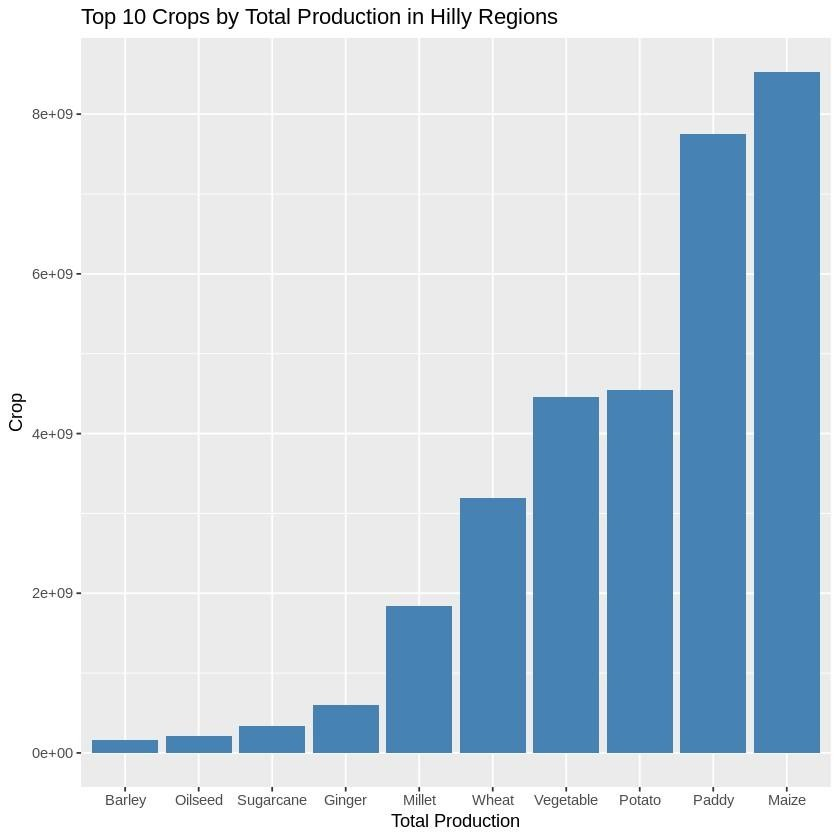
\includegraphics[width=0.5\textwidth]{figures/bar_agri.jpg}
\caption{ Top 10 Crops by Total Production in Hilly Region}
\end{figure}

The resulting plot clearly highlights the dominant crops cultivated in Nepal’s hilly regions. This insight is particularly valuable for stakeholders aiming to understand regional agricultural strengths or to design policies that support the most productive crops in these areas. Maize and Paddy are highly cultivated compared to others in hilly region.

\subparagraph*{Visualization of Agricultural Production by Crop Type in Hilly Districts
}
To understand the overall composition of agricultural production in the hilly districts, we visualize how different crop types contribute to production across various districts. This is done using a stacked bar chart, where each bar represents a district, and the stacked segments represent crop types.

\begin{verbatim}
ggplot(merged_data, aes(x = District, y = Production, fill = Crop.Type)) +
  geom_bar(stat = "identity", position = "stack") +
  coord_flip()
\end{verbatim}

% Figure here-----------------------------
\begin{figure}[h]
\centering
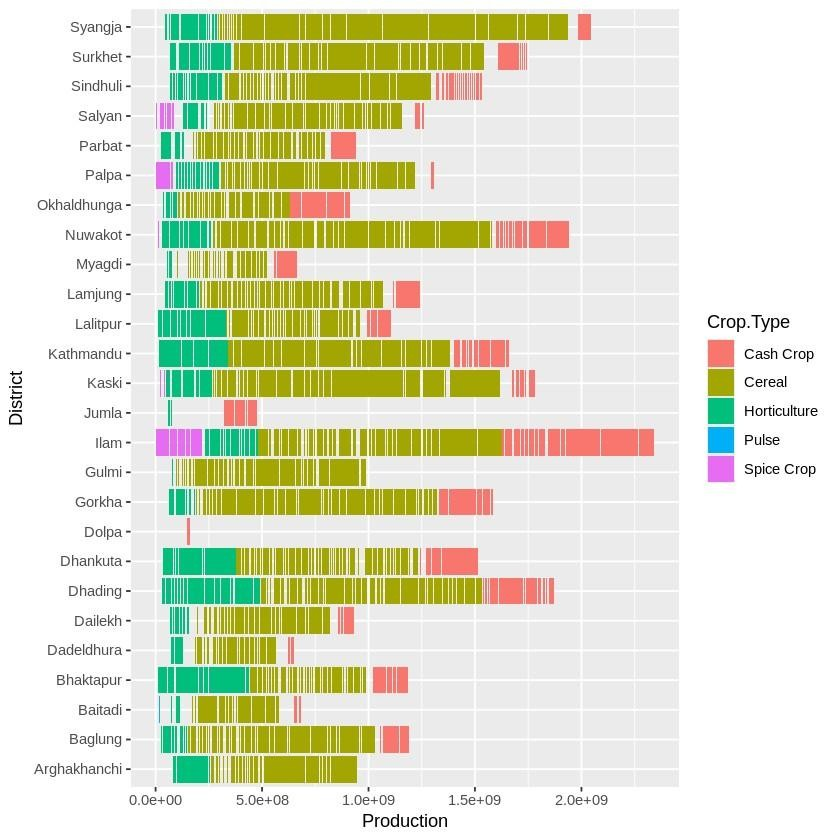
\includegraphics[width=0.6\textwidth]{figures/stacked_agri.jpg}
\caption{Stacked Barchart with crop type production in different districts}
\end{figure}

This visualization helps us compare which crop types dominate production in each district, and whether some regions have a more diverse agricultural profile than others. From the chart we can we that cereal production is highly dominating over hilly region.

\subsection*{Trend Analysis Over Time for Top 5 Crops}

To analyze how production of the most significant crops has changed over time in the hilly regions, we summarize and visualize the yearly production trends for the top 5 crops.

\begin{verbatim}
# Summarize yearly production for top crops
top_crops_list <- head(top_crops$Crop, 5)  # top 5 crops
yearly_trends <- merged_data %>%
  filter(Crop %in% top_crops_list) %>%
  group_by(Year, Crop) %>%
  summarise(Yearly_Production = sum(Production, na.rm = TRUE))
# Plot
ggplot(yearly_trends, aes(x = Year, y = Yearly_Production, color = Crop)) +
  geom_line(linewidth = 1) +
  labs(title = "Yearly Production Trends for Top Crops in Hilly Regions",
       x = "Year",
       y = "Production") +
  theme_minimal()
\end{verbatim}

% Figure here-----------------------------
\begin{figure}[h]
\centering
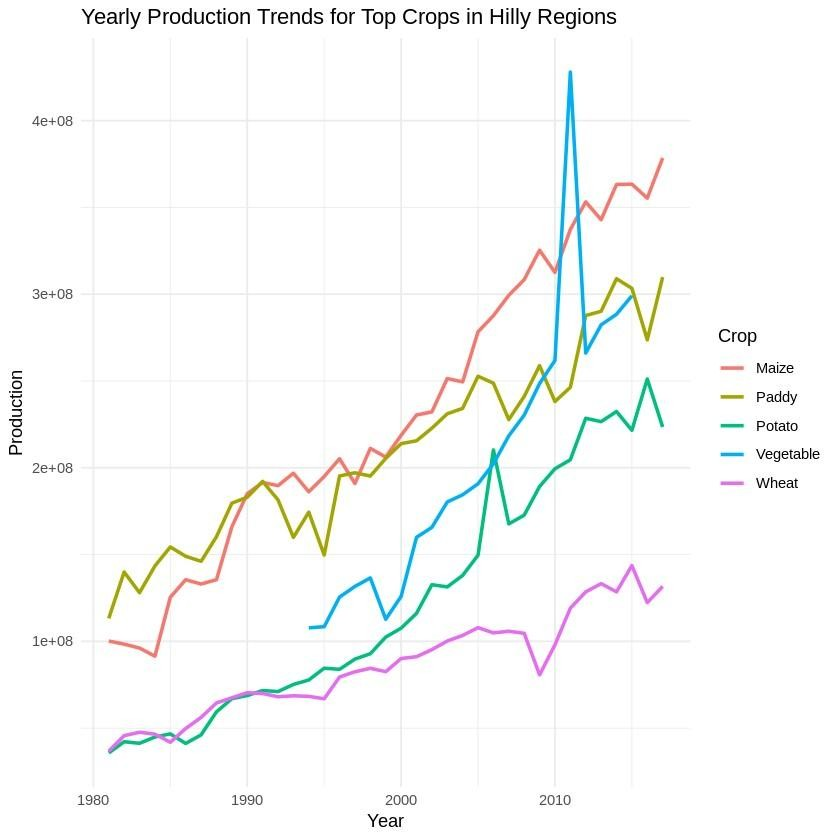
\includegraphics[width=0.5\textwidth]{figures/top5_agri.jpg}
\caption{Trend analysis of Top 5 crops in Hilly}
\end{figure}

\subsection*{Yearly Production of Paddy and Precipitation Trend}

To explore the relationship between agricultural production and climate, we analyze the yearly production of Paddy alongside average precipitation. The following R code aggregates yearly Paddy production and climate data, then plots them with dual y-axes to visualize trends concurrently.

\begin{verbatim}
# Assuming df_paddy_yearly is already created:
df_paddy_yearly <- merged_data %>%
  filter(Crop == "Paddy") %>%
  group_by(Year) %>%
  summarise(
    total_production = sum(Production, na.rm = TRUE),
    avg_temperature = mean(Temp_2m, na.rm = TRUE),
    avg_precip = mean(Precip, na.rm = TRUE)
  )


# Get the max values for dynamic scaling
max_prod_val <- max(df_paddy_yearly$total_production, na.rm = TRUE)
max_precip_val <- max(df_paddy_yearly$avg_precip, na.rm = TRUE)


target_max_proportion <- 0.7


ggplot(df_paddy_yearly, aes(x = Year)) +
  # Line and points for Production
geom_line(aes(y = total_production, color = "Total Production (Kg)"), 
linewidth = 1.2) +
geom_point(aes(y = total_production, color = "Total Production (Kg)"),
size = 3) +

# Line for Precipitation, scaled using the adjusted proportion
geom_line(aes(
  y = avg_precip * (target_max_proportion * max_prod_val / max_precip_val),
  color = "Average Precipitation (mm)"), linewidth = 1.2) +


# Add second axis for Precipitation, using the inverse of the adjusted scaling
scale_y_continuous(
  name = "Total Production (Kg)",
  sec.axis = sec_axis(~ . * (max_precip_val /
   (target_max_proportion * max_prod_val)),name = "Average Precipitation (mm)")
  ) +
# Manually set colors for the lines and define legend labels
scale_color_manual(
  name = "Variable",
  values = c(
      "Total Production (Kg)" = "darkgreen",
      "Average Precipitation (mm)" = "red"
    )
) +
# Titles and labels
labs(
    title = "Yearly Production of Paddy with Precipitation Trend",
    x = "Year"
  ) +
theme_minimal() +
theme(
    axis.text.x = element_text(angle = 45, hjust = 1),
    axis.title.y.left = element_text(color = "darkgreen"),
    axis.title.y.right = element_text(color = "red"),
    legend.position = "bottom",
    legend.title = element_blank(),
    plot.title = element_text(hjust = 0.5, face = "bold")
  )
\end{verbatim}

% Figure here-----------------------------
\begin{figure}[h]
\centering
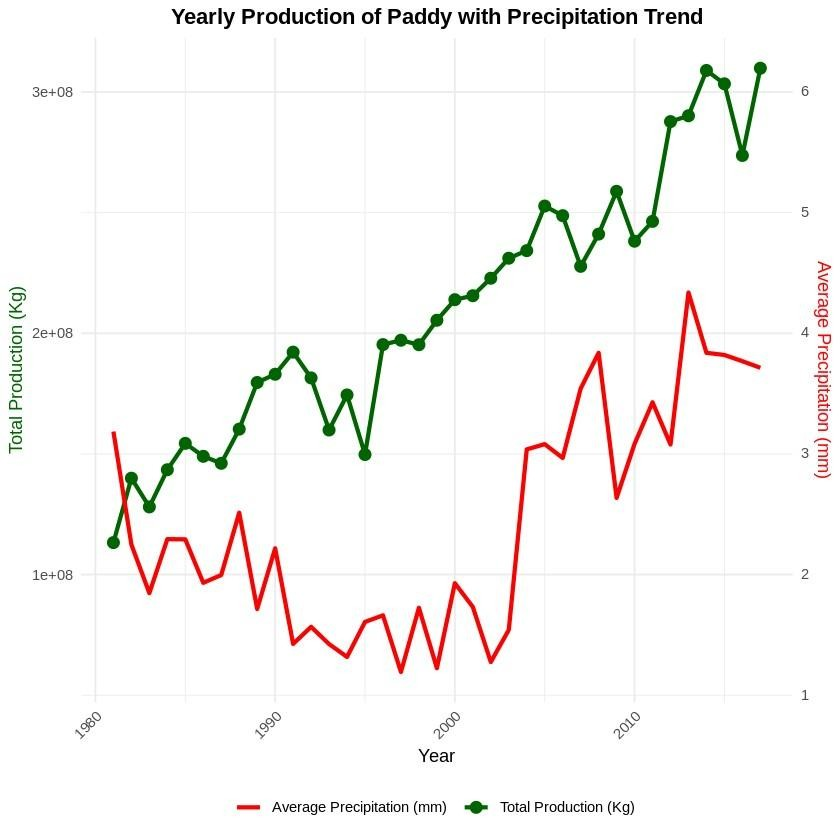
\includegraphics[width=0.5\textwidth]{figures/paddy_trend.jpg}
\caption{Yearly Production of Paddy and Precipitation Trend}
\end{figure}

This plot illustrates how Paddy production varies over the years alongside changes in average precipitation, providing insight into the dependency of agricultural yields on climatic factors in Nepal’s hilly regions. Paddy production has steadily increased over the years, but rainfall shows high variability. Notably, drops in rainfall often correspond to declines in paddy production, highlighting the critical role of adequate rainfall for consistent harvests despite improvements in farming practices.

\subsection*{Correlation Heatmap}

To better understand how climatic factors relate to agricultural outcomes such as crop yield and production, we analyze the correlations between key climate variables and agricultural metrics. This helps reveal any direct linear relationships and the strength of connections within the climate variables themselves. The following code computes and visualizes these correlations using a heatmap.

\begin{verbatim}
library(dplyr)
library(corrplot)
# Step 1: Create a clean numeric dataset for correlation
climate_agri_subset <- aggregated_data %>%
select(avg_temperature, avg_precip, avg_humidity, avg_pressure, avg_wind,
Yield, Production)

# Step 2: Compute correlation matrix
cor_matrix <- cor(climate_agri_subset, use = "complete.obs")

# Step 3: Visualize using corrplot
corrplot(cor_matrix, method = "color",
         type = "upper",        # Only upper triangle
         tl.col = "black",      # Text label color
         addCoef.col = "black", # Add correlation values
         number.cex = 0.7,      # Size of numbers
         col = colorRampPalette(c("red", "white", "blue"))(200))
\end{verbatim}

% Figure here-----------------------------
\begin{figure}[h]
\centering
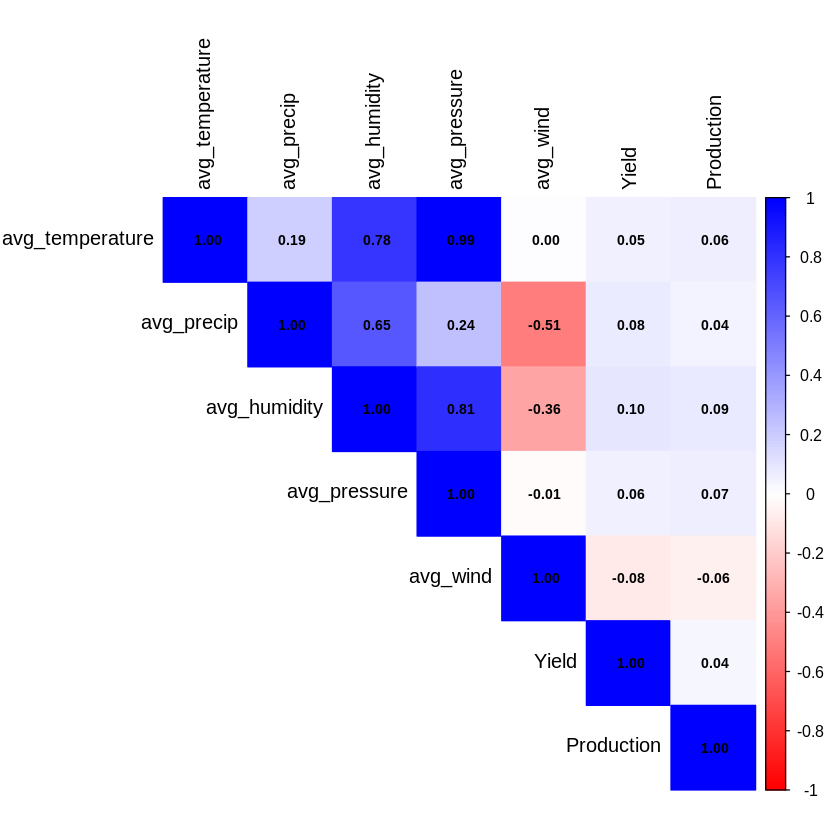
\includegraphics[width=0.5\textwidth]{figures/corr_agri.png}
\caption{Correlation Analysis}
\end{figure}

From this heatmap, several interesting points emerge:

\textbf{Weak Direct Link to Yield and Production:}  
  Correlations between Yield/Production and climate variables (temperature, precipitation, humidity, pressure, wind) are near zero, indicating little to no linear relationship at the annual average level.
  
 \textbf{Why This Matters:}  
 \begin{itemize}
  \item Linear correlation misses non-linear effects (e.g., too much or too little rain affecting yield).  
  \item Annual averages may mask critical seasonal or extreme weather impacts.  
  \item Other factors like technology or irrigation might overshadow climate effects.
 \end{itemize}

 \textbf{Strong Climate Variable Relationships:}  
 \begin{itemize}
  \item Temperature and Pressure: Nearly perfect positive correlation (0.99), suggesting redundancy.  
  \item Humidity: Positively correlated with temperature (0.78) and precipitation (0.65), reflecting natural atmospheric moisture dynamics.  
  \item Wind and Precipitation: Moderately negatively correlated (-0.51), meaning windy years tend to be drier.
 \end{itemize}


